\documentclass{standalone}
\usepackage[usenames,dvipsnames]{xcolor}
\usepackage{amsmath}
\usepackage{amsfonts}
\usepackage{tabularx}
\usepackage{booktabs}
\usepackage{colortbl}
\usepackage{tikz}
\usetikzlibrary{calc}
\pgfdeclarelayer{background}
\pgfdeclarelayer{foreground}
\pgfsetlayers{background,main,foreground}

%\newcommand*\up{\textcolor{green}{%
%  \ensuremath{\blacktriangle}}}
%\newcommand*\down{\textcolor{red}{%
%  \ensuremath{\blacktriangledown}}}
%\newcommand*\const{\textcolor{darkgray}%
%  {\textbf{--}}}
  
\begin{document}

\begin{center}
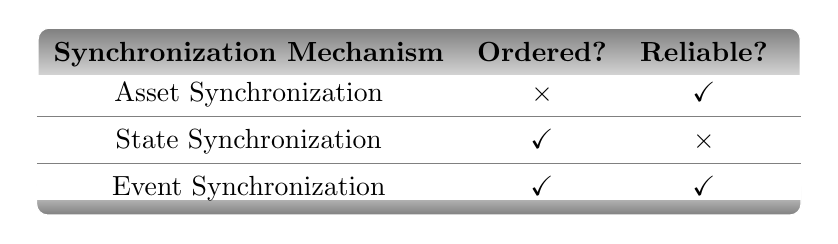
\begin{tikzpicture}
\node (tbl) {
\begin{tabularx}{.8\textwidth}{ccc}
\arrayrulecolor{Gray}
\textbf{Synchronization Mechanism} &
  \textbf{Ordered?} & 
    \textbf{Reliable?} \\
Asset Synchronization\rule{0pt}{2.5ex}  &  $\times$ & \checkmark \\
\midrule
State Synchronization & \checkmark & $\times$ \\
\midrule
Event Synchronization & \checkmark & \checkmark \\
\end{tabularx}
};


\begin{pgfonlayer}{background}
\draw[rounded corners,top color=Gray,bottom color=white,draw=white] ($(tbl.north west)+(0.14,0)$)
    rectangle ($(tbl.north east)-(0.13,0.9)$);
\draw[rounded corners,top color=white,bottom color=Gray,draw=white] ($(tbl.south west)+(0.12,0.5)$) 
    rectangle ($(tbl.south east)-(0.12,0)$);
\draw[top color=white,bottom color=white,draw=white]($(tbl.north east)-(0.13,0.6)$)
    rectangle ($(tbl.south west)+(0.13,0.2)$);
\end{pgfonlayer}


\end{tikzpicture}
\end{center}

\end{document}